\documentclass[tikz,border=14pt]{standalone}
\usepackage[T1]{fontenc}
\usepackage{lmodern}
\usepackage{amsmath,amssymb}
\usetikzlibrary{arrows.meta,positioning,calc,fit,backgrounds,shapes.geometric,shadows}

\newcommand{\ncls}{n_{\mathrm{class}}}

\tikzset{
  marr/.style={-{Stealth[length=2.4mm,width=1.8mm]}, thick, black!70},
  mop/.style={draw, rounded corners=3pt, thick, align=center, minimum height=2.0cm,
              text width=2.3cm, font=\footnotesize, inner sep=3pt},
  mconv/.style={mop, fill=orange!25, draw=orange!70!black},
  mlin/.style={mop, fill=blue!15, draw=blue!60!black},
  mpool/.style={mop, fill=violet!20, draw=violet!70!black},
  mrsh/.style={mop, fill=gray!15, draw=gray!70!black},
  mdrop/.style={mop, fill=red!10, draw=red!60!black, dashed},
  mlstm/.style={mop, fill=teal!20, draw=teal!60!black, text width=1.4cm},
  mact/.style={draw=green!50!black, fill=green!20, circle, thick, font=\scriptsize,
               inner sep=0pt, minimum size=1.05cm, align=center},
  mtens/.style={draw=black!70, thick, fill=yellow!20, font=\scriptsize, align=center,
                double copy shadow={shadow xshift=2.5pt, shadow yshift=2.5pt,
                                    fill=yellow!10, draw=black!60}},
  mvec/.style={draw=black!70, thick, fill=yellow!25, minimum width=0.4cm},
  mdim/.style={font=\scriptsize, align=center, text=black!75},
  msmall/.style={draw, thick, rounded corners=2pt, font=\scriptsize,
                 minimum width=0.9cm, minimum height=0.6cm, fill=white},
  mstage/.style={draw=black!45, dashed, thick, rounded corners=8pt, inner sep=11pt, fill=black!3},
  mstagetitle/.style={font=\bfseries\small},
  mgate/.style={draw, thick, rounded corners=2pt, minimum width=0.95cm,
                minimum height=0.65cm, font=\footnotesize},
  msig/.style={mgate, fill=green!20},
  mthn/.style={mgate, fill=violet!20},
  mopn/.style={draw, circle, thick, inner sep=1pt, minimum size=0.55cm,
               fill=white, font=\footnotesize}
}

\begin{document}
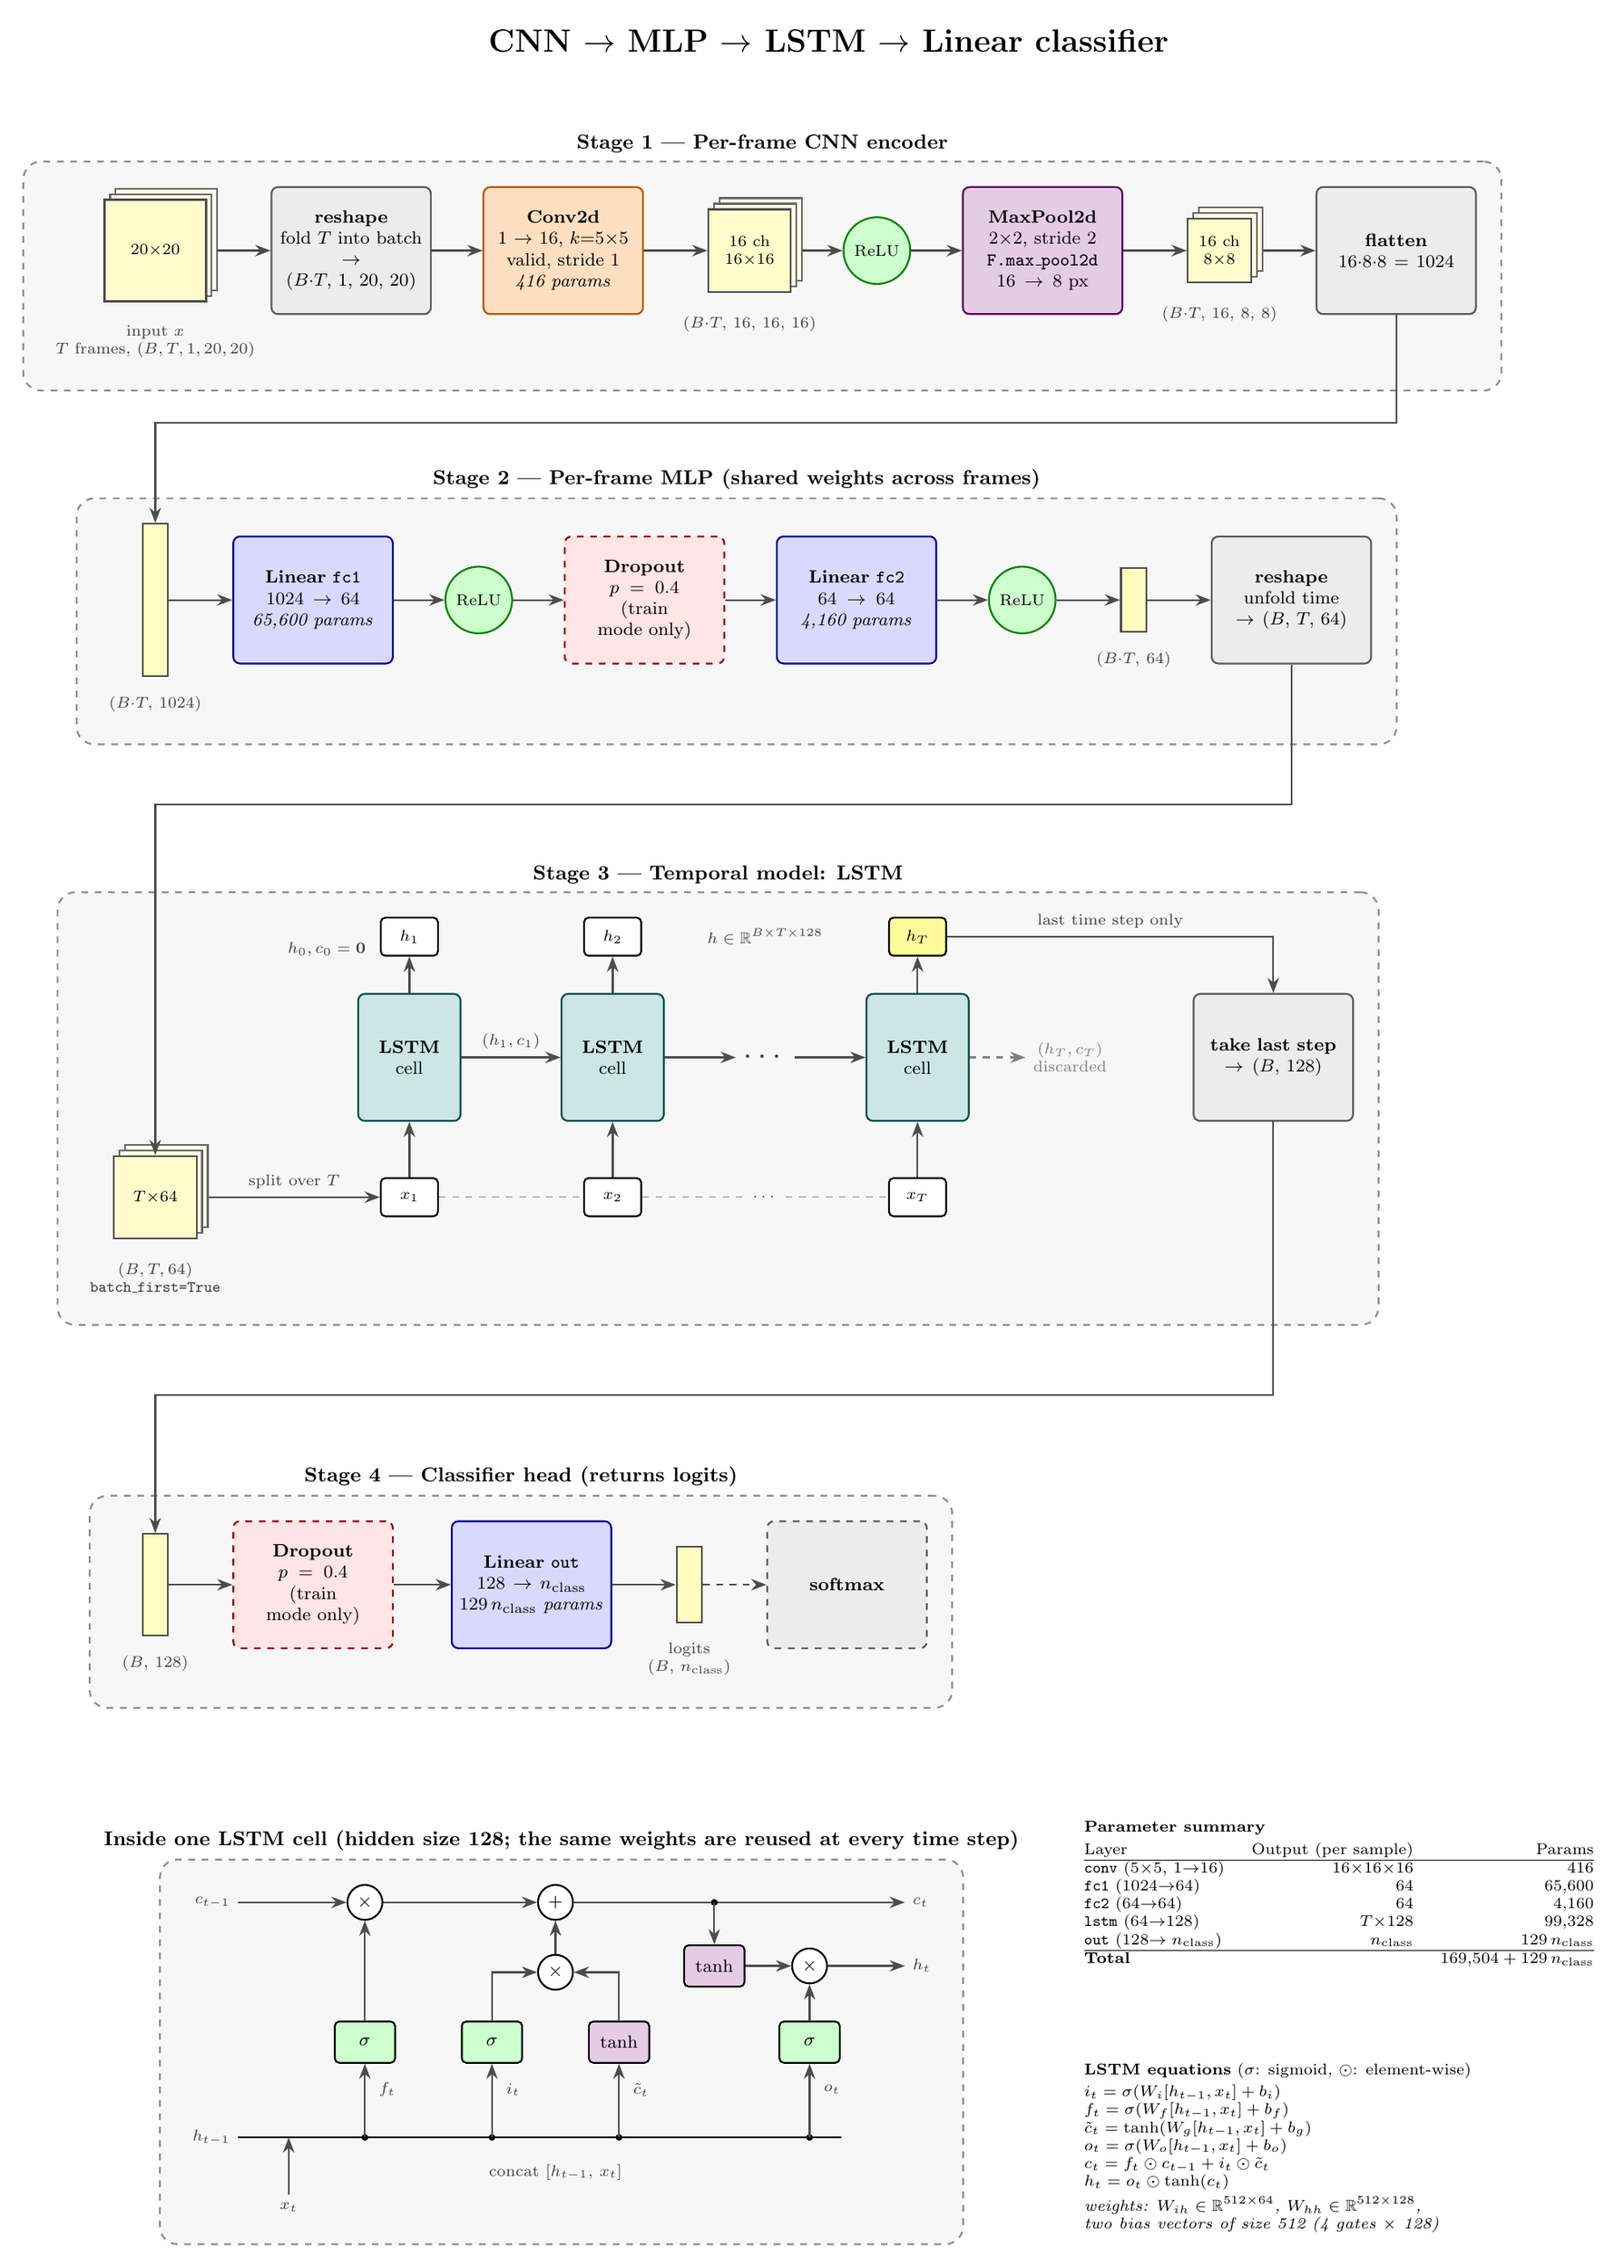
\begin{tikzpicture}[font=\sffamily]

%==================================================================
% TITLE
%==================================================================
\node[font=\Large\bfseries] at (10.6,3.3)
  {CNN $\rightarrow$ MLP $\rightarrow$ LSTM $\rightarrow$ Linear classifier};

%==================================================================
% STAGE 1 : per-frame CNN encoder     (y = 0)
%==================================================================
\node[mtens, minimum size=1.6cm] (inp) at (0,0) {$20{\times}20$};
\node[mrsh, right=1.0cm of inp] (rs1)
  {\textbf{reshape}\\ fold $T$ into batch\\ $\rightarrow(B{\cdot}T,\,1,\,20,\,20)$};
\node[mconv, right=0.8cm of rs1] (cv)
  {\textbf{Conv2d}\\ $1\rightarrow16$, $k{=}5{\times}5$\\ valid, stride 1\\ \textit{416 params}};
\node[mtens, minimum size=1.3cm, right=1.0cm of cv] (fm1) {16 ch\\ $16{\times}16$};
\node[mact, right=0.8cm of fm1] (r1) {ReLU};
\node[mpool, right=0.8cm of r1] (mp)
  {\textbf{MaxPool2d}\\ $2{\times}2$, stride 2\\ \texttt{F.max\_pool2d}\\ $16\rightarrow8$ px};
\node[mtens, minimum size=1.0cm, right=1.0cm of mp] (fm2) {16 ch\\ $8{\times}8$};
\node[mrsh, right=1.0cm of fm2] (fl)
  {\textbf{flatten} $16{\cdot}8{\cdot}8=1024$};

\node[mdim, below=7pt of inp] (l1) {input $x$\\ $T$ frames, $(B,T,1,20,20)$};
\node[mdim, below=7pt of fm1] (l2) {$(B{\cdot}T,\,16,\,16,\,16)$};
\node[mdim, below=7pt of fm2] (l3) {$(B{\cdot}T,\,16,\,8,\,8)$};

\draw[marr] ([xshift=5pt]inp.east) -- (rs1.west);
\draw[marr] (rs1.east) -- (cv.west);
\draw[marr] (cv.east) -- (fm1.west);
\draw[marr] ([xshift=5pt]fm1.east) -- (r1.west);
\draw[marr] (r1.east) -- (mp.west);
\draw[marr] (mp.east) -- (fm2.west);
\draw[marr] ([xshift=5pt]fm2.east) -- (fl.west);

%==================================================================
% STAGE 2 : per-frame MLP             (y = -5.5)
%==================================================================
\node[mvec, minimum height=2.4cm] (v1) at (0,-5.5) {};
\node[mdim, below=5pt of v1] (lv1) {$(B{\cdot}T,\,1024)$};
\node[mlin, right=1.0cm of v1] (fc1)
  {\textbf{Linear} \texttt{fc1}\\ $1024\rightarrow64$ \textit{65,600 params}};
\node[mact, right=0.8cm of fc1] (r2) {ReLU};
\node[mdrop, right=0.8cm of r2] (dr1) {\textbf{Dropout}\\ $p=0.4$\\ (train mode only)};
\node[mlin, right=0.8cm of dr1] (fc2)
  {\textbf{Linear} \texttt{fc2}\\ $64\rightarrow64$\\  \textit{4,160 params}};
\node[mact, right=0.8cm of fc2] (r3) {ReLU};
\node[mvec, minimum height=1.0cm, right=1.0cm of r3] (v2) {};
\node[mdim, below=5pt of v2] (lv2) {$(B{\cdot}T,\,64)$};
\node[mrsh, right=1.0cm of v2] (rs2)
  {\textbf{reshape}\\ unfold time\\ $\rightarrow(B,\,T,\,64)$};

\draw[marr] (v1.east) -- (fc1.west);
\draw[marr] (fc1.east) -- (r2.west);
\draw[marr] (r2.east) -- (dr1.west);
\draw[marr] (dr1.east) -- (fc2.west);
\draw[marr] (fc2.east) -- (r3.west);
\draw[marr] (r3.east) -- (v2.west);
\draw[marr] (v2.east) -- (rs2.west);

% stage 1 -> stage 2
\draw[marr] (fl.south) -- ++(0,-1.7) -| (v1.north);

%==================================================================
% STAGE 3 : LSTM, unrolled            (y = -12.7)
%==================================================================
\node[mtens, minimum size=1.3cm] (seq) at (0,-14.9) {$T{\times}64$};
\node[mdim, below=7pt of seq] (lseq) {$(B,T,64)$\\ \texttt{batch\_first=True}};

\node[mlstm] (c1) at (4.0,-12.7)  {\textbf{LSTM}\\ cell};
\node[mlstm] (c2) at (7.2,-12.7)  {\textbf{LSTM}\\ cell};
\node[mdim]  (cd) at (9.6,-12.7)  {\Large$\cdots$};
\node[mlstm] (cT) at (12.0,-12.7) {\textbf{LSTM}\\ cell};

\node[msmall] (x1) at (4.0,-14.9)  {$x_1$};
\node[msmall] (x2) at (7.2,-14.9)  {$x_2$};
\node[mdim]   (xd) at (9.6,-14.9)  {$\cdots$};
\node[msmall] (xT) at (12.0,-14.9) {$x_T$};

\node[msmall] (h1) at (4.0,-10.8)  {$h_1$};
\node[msmall] (h2) at (7.2,-10.8)  {$h_2$};
\node[mdim]   (hd) at (9.6,-10.8)  {$h\in\mathbb{R}^{B\times T\times128}$};
\node[msmall, fill=yellow!40] (hT) at (12.0,-10.8) {$h_T$};

\node[mdim] (init) at (2.7,-11) {$h_0,c_0=\mathbf{0}$};
\node[mdim, text=gray] (fin) at (14.4,-12.7) {$(h_T,c_T)$\\ discarded};
\node[mrsh] (sel) at (17.6,-12.7)
  {\textbf{take last step} $\rightarrow(B,\,128)$};

% inputs
\draw[marr] ([xshift=5pt]seq.east) -- node[above, mdim] {split over $T$} (x1.west);
\draw[dashed, gray] (x1.east) -- (x2.west);
\draw[dashed, gray] (x2.east) -- (xd.west);
\draw[dashed, gray] (xd.east) -- (xT.west);
\draw[marr] (x1.north) -- (c1.south);
\draw[marr] (x2.north) -- (c2.south);
\draw[marr] (xT.north) -- (cT.south);
% recurrence
\draw[marr] (c1.east) -- node[above, mdim] {$(h_1,c_1)$} (c2.west);
\draw[marr] (c2.east) -- (cd.west);
\draw[marr] (cd.east) -- (cT.west);
%\draw[marr] (init.east) -| ([xshift=6pt]c1.north west);
% outputs
\draw[marr] (c1.north) -- (h1.south);
\draw[marr] (c2.north) -- (h2.south);
\draw[marr] (cT.north) -- (hT.south);
\draw[marr, gray, dashed] (cT.east) -- (fin.west);
\draw[marr] (hT.east) -| node[near start, above, mdim] {last time step only} (sel.north);

% stage 2 -> stage 3
\draw[marr] (rs2.south) -- ++(0,-2.2) -| (seq.north);

%==================================================================
% STAGE 4 : classifier head           (y = -21)
%==================================================================
\node[mvec, minimum height=1.6cm] (v3) at (0,-21) {};
\node[mdim, below=5pt of v3] (lv3) {$(B,\,128)$};
\node[mdrop, right=1.0cm of v3] (dr2) {\textbf{Dropout}\\ $p=0.4$\\ (train mode only)};
\node[mlin, right=0.9cm of dr2] (fco)
  {\textbf{Linear} \texttt{out}\\ $128\rightarrow\ncls$ \textit{$129\,\ncls$ params}};
\node[mvec, minimum height=1.2cm, right=1.0cm of fco] (v4) {};
\node[mdim, below=5pt of v4] (lv4) {logits\\ $(B,\,\ncls)$};
\node[mrsh, dashed, right=1.0cm of v4] (loss)
  {\textbf{softmax}};

\draw[marr] (v3.east) -- (dr2.west);
\draw[marr] (dr2.east) -- (fco.west);
\draw[marr] (fco.east) -- (v4.west);
\draw[marr, dashed] (v4.east) -- (loss.west);

% stage 3 -> stage 4
\draw[marr] (sel.south) -- ++(0,-4.3) -| (v3.north);

%==================================================================
% STAGE 5 : inside one LSTM cell
%==================================================================
\begin{scope}[shift={(1.8,-29.0)}]
  % gates
  \node[msig] (fg) at (1.5,0.8) {$\sigma$};
  \node[msig] (ig) at (3.5,0.8) {$\sigma$};
  \node[mthn] (gg) at (5.5,0.8) {$\tanh$};
  \node[msig] (og) at (8.5,0.8) {$\sigma$};
  \node[mdim, anchor=west] at (1.6,0.05)  {$f_t$};
  \node[mdim, anchor=west] at (3.6,0.05)  {$i_t$};
  \node[mdim, anchor=west] at (5.6,0.05)  {$\tilde{c}_t$};
  \node[mdim, anchor=west] at (8.6,0.05)  {$o_t$};

  % point-wise operations
  \node[mopn] (m1) at (1.5,3.0) {$\times$};
  \node[mopn] (pl) at (4.5,3.0) {$+$};
  \node[mopn] (m2) at (4.5,1.9) {$\times$};
  \node[mthn] (th) at (7.0,2.0) {$\tanh$};
  \node[mopn] (m3) at (8.5,2.0) {$\times$};

  % states in / out
  \node[mdim, anchor=east] (cprev) at (-0.5,3.0) {$c_{t-1}$};
  \node[mdim, anchor=west] (ct)    at (10.0,3.0) {$c_t$};
  \node[mdim, anchor=west] (ht)    at (10.0,2.0) {$h_t$};
  \node[mdim, anchor=east] (hprev) at (-0.5,-0.7) {$h_{t-1}$};
  \node[mdim]              (xt)    at (0.3,-1.8) {$x_t$};

  % cell-state highway
  \draw[marr] (cprev.east) -- (m1.west);
  \draw[marr] (m1.east) -- (pl.west);
  \draw[marr] (pl.east) -- (ct.west);
  \fill (7,3.0) circle (1.5pt);
  \draw[marr] (7,3.0) -- (th.north);

  % gates -> operations
  \draw[marr] (fg.north) -- (m1.south);
  \draw[marr] (ig.north) |- (m2.west);
  \draw[marr] (gg.north) |- (m2.east);
  \draw[marr] (m2.north) -- (pl.south);
  \draw[marr] (th.east) -- (m3.west);
  \draw[marr] (og.north) -- (m3.south);
  \draw[marr] (m3.east) -- (ht.west);

  % concatenated input bus
  \draw[thick] (hprev.east) -- (9.0,-0.7);
  \draw[marr] (xt.north) -- (0.3,-0.7);
  \foreach \xx/\gt in {1.5/fg, 3.5/ig, 5.5/gg, 8.5/og}{
    \fill (\xx,-0.7) circle (1.5pt);
    \draw[marr] (\xx,-0.7) -- (\gt.south);
  }
  \node[mdim] at (4.5,-1.25) {concat $[h_{t-1},\,x_t]$};
\end{scope}

%==================================================================
% LEGEND (right of stage 4)
%==================================================================


%==================================================================
% PARAMETER TABLE + EQUATIONS (right of stage 5)
%==================================================================
\node[anchor=north west, font=\scriptsize, align=left] at (14.5,-24.6) {%
  \textbf{Parameter summary}\\[2pt]
  \begin{tabular}{@{}lrr@{}}
    Layer & Output (per sample) & Params \\ \hline
    \texttt{conv} (5$\times$5, 1$\rightarrow$16) & $16{\times}16{\times}16$ & 416 \\
    \texttt{fc1} (1024$\rightarrow$64)           & 64                       & 65,600 \\
    \texttt{fc2} (64$\rightarrow$64)             & 64                       & 4,160 \\
    \texttt{lstm} (64$\rightarrow$128)           & $T{\times}128$           & 99,328 \\
    \texttt{out} (128$\rightarrow\ncls$)         & $\ncls$                  & $129\,\ncls$ \\ \hline
    \textbf{Total} &  & $169{,}504+129\,\ncls$
  \end{tabular}};

\node[anchor=north west, font=\scriptsize, align=left] at (14.5,-28.4) {%
  \textbf{LSTM equations} ($\sigma$: sigmoid, $\odot$: element-wise)\\[2pt]
  $i_t=\sigma(W_{i}[h_{t-1},x_t]+b_i)$\\
  $f_t=\sigma(W_{f}[h_{t-1},x_t]+b_f)$\\
  $\tilde{c}_t=\tanh(W_{g}[h_{t-1},x_t]+b_g)$\\
  $o_t=\sigma(W_{o}[h_{t-1},x_t]+b_o)$\\
  $c_t=f_t\odot c_{t-1}+i_t\odot\tilde{c}_t$\\
  $h_t=o_t\odot\tanh(c_t)$\\[2pt]
  \textit{weights: $W_{ih}\in\mathbb{R}^{512\times64}$, $W_{hh}\in\mathbb{R}^{512\times128}$,}\\
  \textit{two bias vectors of size 512 (4 gates $\times$ 128)}};

%==================================================================
% STAGE FRAMES (drawn on the background layer)
%==================================================================
\begin{scope}[on background layer]
  \node[mstage, fit=(inp)(fl)(l1)(l2)(l3),
        label={[mstagetitle]above:Stage 1 --- Per-frame CNN encoder}] {};
  \node[mstage, fit=(v1)(rs2)(lv1)(lv2),
        label={[mstagetitle]above:Stage 2 --- Per-frame MLP (shared weights across frames)}] {};
  \node[mstage, fit=(seq)(lseq)(c1)(cT)(x1)(xT)(h1)(hT)(init)(sel)(fin)(hd),
        label={[mstagetitle]above:Stage 3 --- Temporal model: LSTM}] {};
  \node[mstage, fit=(v3)(lv3)(loss)(lv4)(fco),
        label={[mstagetitle]above:Stage 4 --- Classifier head (returns logits)}] {};
  \node[mstage, fit=(cprev)(ct)(ht)(hprev)(xt)(fg)(og)(m1)(th),
        label={[mstagetitle]above:Inside one LSTM cell
               (hidden size 128; the same weights are reused at every time step)}] {};
\end{scope}

\end{tikzpicture}
\end{document}
